\documentclass[]{article}
% So the first line in the section will be indented
\usepackage{indentfirst}
% For the pie chart
\usepackage{pgf-pie}
% For line braks in tables
\usepackage{tabularx}

%opening
\title{Research plan}
\author{Kinga Andrea Gémes}

\begin{document}

\maketitle

\section{Rationale datasets}

The first rationale focused dataset was Movie-rationales annotated by~\cite{Zaidan:2007} and later updated in~\cite{Zaidan:2008}.

\subsection{EREASER collection}

The EREASER~\cite{DeYoung:2020} dataset has been comprised from the following datasets:

\begin{itemize}
	\item FEVER~\cite{Thorne:2018}: Dataset with claims generated by modifying Wikipedia sentences, that have been supported or refuted by Wikipedia article snippets without knowledge of the original sentence,
	\item e-SNLI~\cite{Camburu:2018}: Premise-Hypothesis pairs with rationales for explanation of entailment, neutral, or contradiction relation. Interestingly there are typical cases of explanations, where the reasoning is "just because x, doesn't mean y". From the article: "For entailment, we required justifications of all the parts of the hypothesis that do not appear in the premise. For neutral and contradictory pairs, while we encouraged stating all the
	elements that contribute to the relation, we consider an explanation correct, if at least one element is stated. Finally, we asked the annotators to provide self-contained explanations, as opposed to
	sentences that would make sense only after reading the premise and hypothesis",
	\item Evidence-Inference~\cite{DeYoung:2020b}: Full-text articles annotated with Intervention-Comparator-Outcome triplets which are the prompts (max. 5 prompts/article). These are annotated with increase, decrease, no difference or invalid prompt tags as well as rationales that support the label,
	\item BoolQ~\cite{Clark:2019}: Yes/No question answering task with Wikipedia exerts as the rationale behind the answer, 
	\item CoS-E~\cite{Rajani:2019}: Commonsense reasoning task based on the CQA (Commonsense Question Answering) dataset; their model is made up of two parts: first they train a finetuned language model (GPT) based generator model, that can generate the explanations, than they train on CQA with the added reasoning as an input,
	\item Movie-rationales~\cite{Zaidan:2007,Zaidan:2008}: The authors reannotated an IMDb sentiment polarity dataset with rational labels, the utilized the rationals in a discriminative and generative model (SVM and log-linear respectively), 
	\item Multi-RC~\cite{Khashabi:2018}: Multi-choice question answering task, where at least one answer is correct with a paragraph of context provided,
	\item SciFact~\cite{Wadden:2020}: claims paired with paper abstracts, that support or refute them with rationale annotation in the abstracts.
\end{itemize}

\subsection{Hate speech related datasets}

HateXplain~\cite{Mathew:2021} is a dataset with three main labels: hateful, offensive and neutral as well as multiple target categories.

M-Phasis~\cite{Ruiter:2022} is a feature annotated dataset (no rationales, but with features like mentions of x group of people in a positive/negative light) in French and German.

WikiAttack~\cite{Carton:2018} is a dataset with Wikipedia comments that have been removed for toxicity, personal attacks or aggression. The later rationale annotation added highlights to personal attacks. They used an adversarial structure, similar to GAN.

\subsection{Other datasets}

ComVE~\cite{Wang:2019} contains an assortment of statements, each either making sense or not. If the statement does not make sense, there is rationale provided as for why.

Stanford Sentiment Treebank (SST)~\cite{Socher:2013} is a sentiment labeled treebank that can be used for sentiment analysis with the rationales being the node sentiments.

BeerAdvocate~\cite{McAuley:2012} is a dataset of Beer reviews where the different aspects on the reviews (feel, look, smell, taste) are highlighted in the text and this might be used to predict the overall score easier.

\cite{Wiegreffe:2021} collected and analyzed multiple datasets with rationales.

\clearpage

\subsection{Dataset categories}

\begin{center}
	\begin{table}[!ht]
		\footnotesize
		\begin{tabularx}{\linewidth}{XllX}
			\textbf{Dataset}&\textbf{Type}&\textbf{Topic}&\textbf{Medium} \\ \hline
			Movie-rationales \cite{Zaidan:2008}&Sentiment&Review&IMDb \\
			BeerAdvocate \cite{McAuley:2012}&Sentiment&Review&Multi (BeerAdvocate, Audible, etc.) \\
			SST \cite{Socher:2013}&Sentiment&Review&Previous Dataset; Movie Reviews \\
			FEVER \cite{Thorne:2018}&Reasoning&Every Day&Wikipedia \\
			e-SNLI \cite{Camburu:2018}&Entailment&Every Day&Previous Dataset; SNLI \\
			Multi-RC \cite{Khashabi:2018}&Question Answering&Every Day&Multi (News, Wikipedia, etc.) \\
			WikiAttack \cite{Carton:2018}&Hate Speech&Hate&Wikipedia \\
			BoolQ \cite{Clark:2019}&Question Answering&Every Day&Wikipedia \\
			CoS-E \cite{Rajani:2019}&Question Answering&Common Sense&Previous Dataset; Hand Written \\
			ComVE \cite{Wang:2019}&Reasoning&Common Sense&Hand Written \\
			Evidence-Inference \cite{DeYoung:2020b}&Reasoning&Scientific&Scientific Papers \\
			SciFact \cite{Wadden:2020}&Reasoning&Scientific&Scientific Papers \\
			HateXplain \cite{Mathew:2021}&Hate Speech&Hate&Social Media \\
			M-Phasis \cite{Ruiter:2022}&Hate Speech&Hate&Social Media \\
		\end{tabularx}
	\caption{Datasets annotated with rationales ordered by the publication date}
	\label{tab:dataset}
	\end{table}
\end{center}


\begin{figure}[!ht]
	\footnotesize
	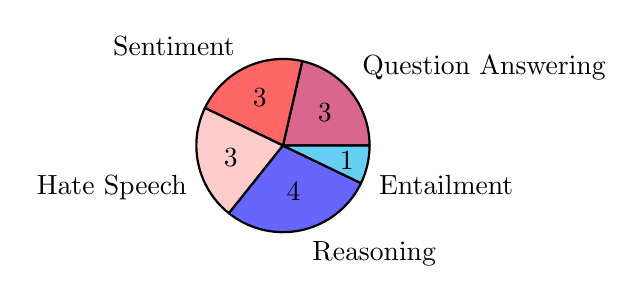
\begin{tikzpicture}[scale=0.55]
	\centering\pie[/tikz/every pin/.style={align=center}, radius=2, sum = auto,
	color = {purple!60!white, red!60!white, pink!80!white, blue!60!white, cyan!60!white}, explode={0, 0, 0, 0, 0}]{3/Question Answering, 3/Sentiment, 3/Hate Speech, 4/Reasoning, 1/Entailment};
	\end{tikzpicture}\qquad
	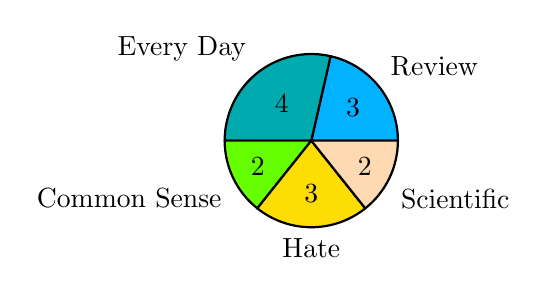
\begin{tikzpicture}[scale=0.55]
	\centering\pie[/tikz/every pin/.style={align=center}, radius=2, sum = auto,
	color = {blue!30!cyan, cyan!60!green, green!60!yellow, yellow!80!orange, orange!30!white}, explode={0, 0, 0, 0, 0}]{3/Review, 4/Every Day, 2/Common Sense, 3/Hate, 2/Scientific};
	\end{tikzpicture}
	\caption{The type and topic distribution of the above mentioned datasets}
	\label{fig:dataset}
\end{figure}

\clearpage

\section{Evaluations}

We can evaluate the correctness predicted rationales by contrasting it to the reference rationales as well as using certain methods to measure faithfulness even in the absence of true rationales.

\subsection{Metrics}

The metrics are defined in~\cite{DeYoung:2020}. These metrics are: Plausibility with token level precision, recall and f-score as well as intersection over union (IOU) measure, which is a partial matching method, and faithfulness, which has two parts: comprehensiveness (did we really need all of these?) and sufficiency (is there enough rationale given to support the decision?)

\[IOU\_TP = \frac{|predicted\ rationales \cap true\ rationales|}{|predicted\ rationales \cup true\ rationales|} >= 0.5\]

\[hard\_token\_prec = \frac{|predicted\ rationales \cap true\ rationales|}{|predicted\ rationales|}\]

\[hard\_token\_rec = \frac{|predicted\ rationales \cap true\ rationales|}{|true\ rationales|}\]

\[comprehensiveness = model\_output(text)\ -\ model\_output(text\ -\ predicted\ rationales) \]

\[sufficiency = model\_output(text)\ -\ model\_output(predicted\ rationales)\]

\subsection{Human rationales}

Evaluating human rationales \cite{Carton:2020}

The conclusion of the paper is that "from a model accuracy perspective, the quality of human rationales is strong for FEVER, MultiRC, and Movie, mixed for E-SNLI, and poor for SST and WikiAttack."

\section{Explaining systems}

\subsection{Rationale generation before label prediction}

Most datasets described previously provide a baseline solution and most of them used the rationales as an input, or similar to attention, and defined a generator to choose the rationales.

\cite{Lei:2016} presented the problem like information retrieval. Their model is an Encoder-Generator model, with an RCNN core. They trained the model on the BeerAdvocate dataset as well as the AskUbuntu~\cite{dosSantos:2015} data, which contains AskUbuntu questions with similar question pairings. This paper has proven to be influential in the field. The rationale generation model proposed here has been updated to a BERT-to-BERT form by \cite{DeYoung:2020}. This has been further developed by \cite{Carton:2022}, who applied additional tricks for learning from rationales, such as class weighting with attention to rationales, sentence level rationalization, using importance embeddings, and selectively supervising only on human rationales.

\cite{Jain:2020} also uses the same Encoder-Generator model, passing only the extracted, encoded parts of the input through the later half of the model. They applied a feature importance scoring (based on BERT self-attention) trick to be able to train the two parts of the network separately.

Extractive reasoning has been applied by \cite{Zhang:2021}. Their model has been trained on Movie-reviews, FEVER, and Multi-RC. The model itself is based on BERT with added LSTM.

\cite{Majumder:2021} focuses on solving commonsense tasks. They used COMET~\cite{Bosselut:2019} as the commonsense information. The system extracts rationales, which it passes to the commonsense knowledge module, which in turn passes the connected knowledge to a selector. The selected knowledge is passed through a natural language explainer with a final predictor at the end. It has been trained on ComVE, CoS-E, and e-SNLI as well as visual media. They have experimented with replacing COMET with ConceptNet, but it returned only \(\frac{3}{4}\) as much commonsense knowledge for the queries.

Saliency maps are contrasted with influence functions by \cite{Han:2020}. They show the usage of influence functions on sentiment analysis and NLI tasks. Influence functions show the importance of training examples in contrast to saliency maps, which measure token level importance. They observed, that the density of highly influential tokens correlates with the impact of the training sample, thus concluding that saliency maps and influence functions can be used together. Influence functions can also be used to measure correlation of observed data artifacts and influential training examples.

\subsection{Post-hoc explanation}

We can distinguish between two main explaining methods that can be used after the model has been trained. The first and most straight forward method is perturbation, meaning that we modify the input (by removing, masking, or altering parts of it) and observe how the model's output changes with each modification. This is a very time intensive task depending on the model's size and the input modifications.

Perturbation based post-hoc explaining systems treat the model in question as a black box. The most well known post-hoc explaining system is LIME~\cite{Ribeiro:2016}, which provides locally faithful explanations for the given input, similar to saliency maps. An extension and improvement of this model is SHAP~\cite{Lundberg:2017}, which incorporates Shapley values into the prediction to ensure local accuracy, missingness and consistency.

Backpropagation based, or gradient methods utilize one or more forward pass and backpropagation step and use the computed gradients to produce attribution, or saliency maps. One such model is DeepLIFT~\cite{Shrikumar:2017}, which has been designed to work with feed forward neural networks.

\subsubsection{The problem with post-hoc explanation}

The trustworthiness of model explanation methods first came into question by~\cite{Lipton:2018}, and later, more focused on the post-hoc explanation in regards to image classification \cite{Dombrowski:2019}. Soon after \cite{Slack:2020} examined how easy it is to fool LIME and SHAP. The paper describes an adversarial method, that uses an intentionally discriminative model, that makes decisions based on race or gender, as well as non-biased model that uses synthetic features unrelated to sensitive information in criminal case, and credit calculator datasets. It has been able to influence the LIME and to a lesser extent SHAP to behave like the non-biased model when trying to interpret the biased one.

\cite{Krishna:2022} conducted surveys to measure the attitude of data scientist towards the disagreement problem when using post-hoc explanations.

\section{Research Plan}

I plan to run the following experiments on one of the hate speech datasets:

\begin{itemize}
	\item BERT system (most likely RoBERTa, because of its popularity) with post-hoc explanation (LIME os SHAP)
	\item BERT system for rationale generation based on \cite{DeYoung:2020}
	\item Using post-hoc explanation on the model above
	\item Define rule system based on the rationales
	\item Train rule system to expand previous rules to better represent the predictions
	\item Measure fidelity of each model
	\item Measure fidelity of human annotations using the above models
\end{itemize}

\bibliographystyle{apalike}
\bibliography{related_articles.bib}

\end{document}
